%% ;;; -*- mode: Rnw; -*-
\documentclass{config/apuntes}\usepackage[]{graphicx}\usepackage[]{xcolor}
% maxwidth is the original width if it is less than linewidth
% otherwise use linewidth (to make sure the graphics do not exceed the margin)
\makeatletter
\def\maxwidth{ %
  \ifdim\Gin@nat@width>\linewidth
    \linewidth
  \else
    \Gin@nat@width
  \fi
}
\makeatother

\definecolor{fgcolor}{rgb}{0.345, 0.345, 0.345}
\newcommand{\hlnum}[1]{\textcolor[rgb]{0.686,0.059,0.569}{#1}}%
\newcommand{\hlsng}[1]{\textcolor[rgb]{0.192,0.494,0.8}{#1}}%
\newcommand{\hlcom}[1]{\textcolor[rgb]{0.678,0.584,0.686}{\textit{#1}}}%
\newcommand{\hlopt}[1]{\textcolor[rgb]{0,0,0}{#1}}%
\newcommand{\hldef}[1]{\textcolor[rgb]{0.345,0.345,0.345}{#1}}%
\newcommand{\hlkwa}[1]{\textcolor[rgb]{0.161,0.373,0.58}{\textbf{#1}}}%
\newcommand{\hlkwb}[1]{\textcolor[rgb]{0.69,0.353,0.396}{#1}}%
\newcommand{\hlkwc}[1]{\textcolor[rgb]{0.333,0.667,0.333}{#1}}%
\newcommand{\hlkwd}[1]{\textcolor[rgb]{0.737,0.353,0.396}{\textbf{#1}}}%
\let\hlipl\hlkwb

\usepackage{framed}
\makeatletter
\newenvironment{kframe}{%
 \def\at@end@of@kframe{}%
 \ifinner\ifhmode%
  \def\at@end@of@kframe{\end{minipage}}%
  \begin{minipage}{\columnwidth}%
 \fi\fi%
 \def\FrameCommand##1{\hskip\@totalleftmargin \hskip-\fboxsep
 \colorbox{shadecolor}{##1}\hskip-\fboxsep
     % There is no \\@totalrightmargin, so:
     \hskip-\linewidth \hskip-\@totalleftmargin \hskip\columnwidth}%
 \MakeFramed {\advance\hsize-\width
   \@totalleftmargin\z@ \linewidth\hsize
   \@setminipage}}%
 {\par\unskip\endMakeFramed%
 \at@end@of@kframe}
\makeatother

\definecolor{shadecolor}{rgb}{.97, .97, .97}
\definecolor{messagecolor}{rgb}{0, 0, 0}
\definecolor{warningcolor}{rgb}{1, 0, 1}
\definecolor{errorcolor}{rgb}{1, 0, 0}
\newenvironment{knitrout}{}{} % an empty environment to be redefined in TeX

\usepackage{alltt}

\title{Programación y Estadística con R}
\author{Sandra Mingo Ramírez}
\date{2024/25}
\acronym{PRSTR}

\usepackage[all]{nowidow}
\usepackage{listing}
\usepackage{color}
\usepackage{tabularx}
\usepackage{multirow}
\usepackage{makecell}
\usepackage{amsmath}
\usepackage{array}

\newcommand{\code}[1]{\texttt{#1}}



\IfFileExists{upquote.sty}{\usepackage{upquote}}{}
\begin{document}

\begin{abstract}
Este curso es una introducción rápida a un «entorno para la computación estadística y los gráficos», que proporciona una amplia variedad de técnicas estadísticas y gráficas: modelización lineal y no lineal, pruebas estadísticas, análisis de series temporales, clasificación, agrupación, etc. Prácticamente todos los análisis estadísticos que se realizan en Bioinformática se pueden llevar a cabo con R. Además, la «minería de datos» está bien cubierta en R: el clustering (a menudo llamado «análisis no supervisado») en muchas de sus variantes (jerárquico, k-means y familia, modelos de mezcla, fuzzy, etc), bi-clustering, clasificación y discriminación (desde el análisis discriminante a los árboles de clasificación, bagging, máquinas de vectores soporte, etc), todos tienen muchos paquetes en R. Así, tareas como la búsqueda de subgrupos homogéneos en conjuntos de genes/sujetos, la identificación de genes que muestran una expresión diferencial (con ajuste para pruebas múltiples), la construcción de algoritmos de predicción de clases para separar a los pacientes de buen y mal pronóstico en función del perfil genético, o la identificación de regiones del genoma con pérdidas/ganancias de ADN (alteraciones del número de copias) pueden llevarse a cabo en R de forma inmediata.
\end{abstract}

\pagestyle{plain}

\maketitle

\tableofcontents


%Quick intro to R and a minimal of stats
%R programming with a modicum of stats
%Statistics with R: linear models
%Intro to causal inference
%Stats for omics

%Ejercicio de programación (40%) y dos exámenes parciales (30% cada uno)
%Ejercicio de programación en grupos de 3 o 4 personas, presentación de 13 minutos por grupo
%Evitar tidyverse

%09/10 - Ramón Díaz
\chapter{Introducción en R y estadística}
\section{RStudio y primeras nociones}
En RStudio, se puede crear un nuevo fichero en File > New File > R script. Se abre un nuevo fichero en el que se puede programar. En R, la asignación de variables se realiza con <-. En la parte superior derecha, se pueden ver todas las variables que se han asignado en la sesión, los datos y las funciones.

\begin{knitrout}
\definecolor{shadecolor}{rgb}{0.969, 0.969, 0.969}\color{fgcolor}\begin{kframe}
\begin{alltt}
\hldef{x} \hlkwb{<-} \hlnum{9}
\hldef{y} \hlkwb{<-} \hlkwd{matrix}\hldef{(}\hlnum{1}\hlopt{:}\hlnum{20}\hldef{,} \hlkwc{ncol} \hldef{=} \hlnum{4}\hldef{)}
\end{alltt}
\end{kframe}
\end{knitrout}

En la parte inferior derecha hay una pestaña para poder visualizar los gráficos. Desde ese menú, se puede guardar, pero esto no es recomendable, ya que el gráfico se ajusta al tamaño de la pantalla y luego eso no es reproducible. En otra pestaña aparece un listado de todos los paquetes instalados en el disco duro, aunque luego haya que cargarlos en cada script en el que se desee usar. Al pulsar en el nombre de un paquete, se va a la página de ayuda del mismo. También es posible acceder con:

\begin{knitrout}
\definecolor{shadecolor}{rgb}{0.969, 0.969, 0.969}\color{fgcolor}\begin{kframe}
\begin{alltt}
\hlkwd{help}\hldef{(rnorm)}
\end{alltt}
\end{kframe}
\end{knitrout}

La mayor parte del trabajo «real» con R requerirá la instalación de paquetes. Los paquetes proporcionan funcionalidad adicional. Los paquetes están disponibles en muchas fuentes diferentes, pero posiblemente las principales ahora son CRAN y BioConductor. Si un paquete está disponible en CRAN, puedes hacer lo siguiente:

\begin{knitrout}
\definecolor{shadecolor}{rgb}{0.969, 0.969, 0.969}\color{fgcolor}\begin{kframe}
\begin{alltt}
\hlkwd{install.packages}\hldef{(}\hlsng{"nombre-paquete"}\hldef{)} \hlcom{# 1 paquete}
\hlkwd{install.packages}\hldef{(}\hlkwd{c}\hldef{(}\hlsng{"paquete1"}\hldef{,} \hlsng{"paquete2"}\hldef{))} \hlcom{# varios paquetes}
\end{alltt}
\end{kframe}
\end{knitrout}

En Bioinformática, BioConductor es una fuente bien conocida de muchos paquetes diferentes. Los paquetes de BioConductor pueden instalarse de varias maneras, y existe una herramienta semiautomatizada que permite instalar conjuntos de paquetes BioC. Implican hacer algo como

\begin{knitrout}
\definecolor{shadecolor}{rgb}{0.969, 0.969, 0.969}\color{fgcolor}\begin{kframe}
\begin{alltt}
\hldef{BiocManager}\hlopt{::}\hlkwd{install}\hldef{(}\hlsng{"nombre-paquete"}\hldef{)}
\end{alltt}
\end{kframe}
\end{knitrout}

A veces los paquetes dependen de otros paquetes. Si este es el caso, por defecto, los mecanismos anteriores también instalarán las dependencias. Con algunas interfaces gráficas de usuario (en algunos sistemas operativos) también puede instalar paquetes desde una entrada de menú. Por ejemplo, en Windows, hay una entrada en la barra de menú llamada Paquetes, que permite instalar desde Internet, cambiar los repositorios, instalar desde archivos zip locales, etc. Del mismo modo, desde RStudio hay una entrada para instalar paquetes (en «Herramientas»). Los paquetes también están disponibles desde otros lugares (RForge, github, etc); a menudo encontrarás instrucciones allí.

Siempre puedes simplemente matar RStudio; pero eso no es agradable. En todos los sistemas escribir q() en el símbolo del sistema debería detener R/RStudio. También habrá entradas de menú (por ejemplo, «Salir de RStudio» en «Archivo», etc). A continuación sale la pregunta de si se debe guardar el workspace, y en general querremos decir que no.

\section{Ejemplo}
\subsection{Introducción al test de la t}
En un test de la t, la hipótesis nula ($H_0$) suele representar lo contrario de lo que se desea demostrar. Por ejemplo, si nuestro objetivo es comprobar si hay diferencias entre dos muestras, la hipótesis nula establece que ambas son iguales. A continuación, se utiliza la fórmula de la t para obtener un valor estadístico, cuya distribución se examina bajo la suposición de que $H_0$ es cierta. Luego, se calcula la probabilidad de observar un resultado tan extremo o más extremo que el obtenido bajo $H_0$. Esta probabilidad se denomina p-valor, y su interpretación indica cuánta evidencia hay en contra de $H_0$: un p-valor bajo sugiere que lo observado es improbable bajo $H_0$.

\[
t = \frac{x_A - x_B}{SD_{x_A, x_B}}
\]

Es importante aclarar que el p-valor no representa la probabilidad de que $H_0$ sea cierta, ni la probabilidad de que $H_0$ o la hipótesis alternativa ($H_1$) se cumplan dado los datos. Lo que el p-valor señala es que, o bien $H_0$ es falsa, o ha ocurrido un evento tan improbable como el valor observado. No se "rechaza" $H_0$ de manera concluyente, sino que simplemente no se acepta si el p-valor es suficientemente bajo. En este análisis, se compara el resultado observado con todos aquellos más extremos, algo que es distinto de seleccionar el valor que hace los datos lo más probables posible (como se hace en la máxima verosimilitud).

Por ejemplo, una moneda perfectamente equilibrada tiene una probabilidad de $0.5^6$ de que al lanzarla seis veces, salga exactamente tres veces cara y tres veces cruz. Aunque este número es pequeño, no implica que la hipótesis alternativa sea necesariamente más probable, ya que otros resultados también podrían ser igualmente o más improbables. En la mayoría de los casos de comparación de medias, los datos no están restringidos a un único valor.

Cuando $H_0$ es cierta:
$$Pr(p-valor \leq 0,05) = 0,05$$
$$Pr(p-valor \leq 0,01) = 0,01$$

En muchos casos se comprueba más de una $H_0$. En un screening, se analizan 20.000 genes y se decide elegir todos aquellos que tengan un p-valor inferior a 0,05. Esa lista, sobre el total de los genes, la probabilidad de rechazar $H_0$ cuando es cierta, es muy superior al 5\%, aunque se cumpla para cada gen individual. Así, se debe trasladar la lógica al test múltiple, puesto que si no se va a rechazar $H_0$ en muchas ocasiones cuando no se debería.

\subsection{Problema de las pruebas múltiples}
Es posible que hayamos oído hablar del problema de las pruebas múltiples con los microarrays: si observamos los p-valores de un gran número de pruebas, podemos ser inducidos a pensar erróneamente que está ocurriendo algo (es decir, que hay genes expresados de forma diferencial) cuando, en realidad, no hay absolutamente ninguna señal en los datos. A nosotros esto nos convence. Pero tienes un colega testarudo que no lo está. Ha decidido utilizar un ejemplo numérico sencillo para mostrarle el problema. Este es el escenario ficticio: 50 sujetos, de los cuales 30 tienen cáncer y 20 no. Medimos 1000 genes, pero ninguno de los genes tiene diferencias reales entre los dos grupos; para simplificar, todos los genes tienen la misma distribución (una distribución normal). Haremos una prueba t por gen, mostrará un histograma de los valores p e informaremos del número de genes «significativos» (genes con p < 0,05). Este es el código R:

\begin{knitrout}
\definecolor{shadecolor}{rgb}{0.969, 0.969, 0.969}\color{fgcolor}\begin{kframe}
\begin{alltt}
\hldef{randomdata} \hlkwb{<-} \hlkwd{matrix}\hldef{(}\hlkwd{rnorm}\hldef{(}\hlnum{50} \hlopt{*} \hlnum{1000}\hldef{),} \hlkwc{ncol} \hldef{=} \hlnum{50}\hldef{)}
\hldef{class} \hlkwb{<-} \hlkwd{factor}\hldef{(}\hlkwd{c}\hldef{(}\hlkwd{rep}\hldef{(}\hlsng{"NC"}\hldef{,} \hlnum{20}\hldef{),} \hlkwd{rep}\hldef{(}\hlsng{"cancer"}\hldef{,} \hlnum{30}\hldef{)))}
\hldef{pvalues} \hlkwb{<-} \hlkwd{apply}\hldef{(randomdata,} \hlnum{1}\hldef{,}
                 \hlkwa{function}\hldef{(}\hlkwc{x}\hldef{)} \hlkwd{t.test}\hldef{(x} \hlopt{~} \hldef{class)}\hlopt{$}\hldef{p.value)}
\end{alltt}
\end{kframe}
\end{knitrout}

Para leer el código, se empieza por la función más interna, que en este caso es \code{rnorm}. Así, primero se generan 50.000 entradas de distribución normal (1000 genes por 50 personas) de los que se quiere realizar 1000 contrastes de hipótesis (uno por gen) y representar el aspecto de la distribución (que será uniforme). Todas las entradas se organizan en una matriz con 50 columnas. Después, se crean los dos grupos que se están analizando mediante repeticiones (función \code{rep}). El comando de \code{factor} crea las etiquetas. En R, se puede llamar al test de la t de varias maneras, siendo una estándar con la interfaz de tipo fórmula (x $\sim$ class), dividiendo así x en los distintos niveles que se han creado previamente. La sintaxis siempre es una variable que va cambiando (en este caso, las filas) antes de la virgulilla y una variable constante después de la virgulilla (los distintos niveles). La función \code{apply} permite aplicar una función a un objeto o conjunto de datos, evitando así tener que realizar un bucle for. El primer argumento es el objeto, el segundo la dimensión del objeto a lo que se quiere aplicar (si se recorren filas, columnas, etc.), y el tercero la función que se va a aplicar. La función \code{t.test} devuelve objetos a los que se puede acceder, como el valor t, df, p-valor, la media de cada grupo, etc. Se puede acceder al nombre de todos los valores mediante \code{names(t.test(x $\sim$ class))}. En nuestro caso, x es el valor que irá adquiriendo el número de filas a recorrer. En este caso, se define la función en el momento de llamarla, pero también se puede definir antes y utilizarla en el apply. En este caso se define dentro porque es una función corta que solo se utilizará en ese momento, por lo que no es necesario crearla fuera. Si por el contrario fuese una función a la que quisiéramos acceder posteriormente o que fuese compleja con varias líneas, se suele crear fuera. Por último, se accede a los p-valores y se guardan en la variable \code{pvalues}. Esos p-valores se pueden representar a continuación en un histograma y calcular todos aquellos que sean menores o iguales que 0,05.

\begin{knitrout}
\definecolor{shadecolor}{rgb}{0.969, 0.969, 0.969}\color{fgcolor}\begin{kframe}
\begin{alltt}
\hlkwd{hist}\hldef{(pvalues)}
\end{alltt}
\end{kframe}
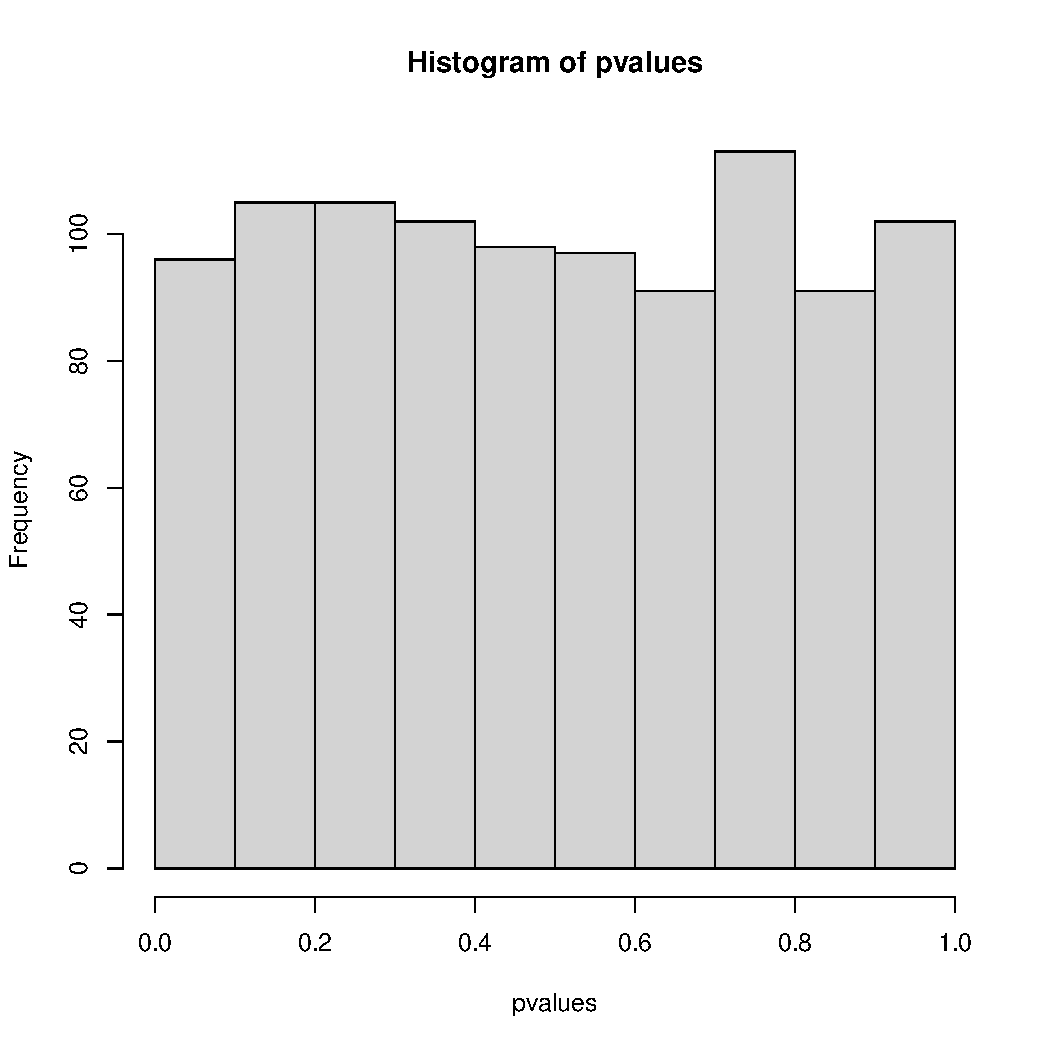
\includegraphics[width=\maxwidth]{figure/unnamed-chunk-7-1} 
\begin{kframe}\begin{alltt}
\hlkwd{sum}\hldef{(pvalues} \hlopt{<=} \hlnum{0.05}\hldef{)}
\end{alltt}
\begin{verbatim}
## [1] 55
\end{verbatim}
\end{kframe}
\end{knitrout}

Al realizar la suma de una lógica booleana, se coercia para que los valores falsos se conviertan en 0 y los verdaderos en 1. Así, al sumarlos, el resultado es numérico. 

En resumen, en este ejemplo hemos visto los siguientes objetos:
\begin{itemize}
\item Vectores: colección de uno o más datos del mismo tipo.
\item Matrices: conjunto de datos indexados por filas y columnas del mismo tipo. 
\item Arrays: generalización de una matriz que no tiene límite de dimensiones (pero debe tener una estrucrtura rectangular). 
\item Data frames: estructura rectangular de dos dimensiones (filas y columnas) en la que cada columna puede ser de un tipo diferente. 
\item Listas: cajón desastre en el que se pueden meter muchas cosas de muchos tipos distintos. Muchas funciones devuelven listas u objetos que contienen listas.
\item Factores: vectores de un tipo especial (variable categórica).
\item Funciones: objetos que realizan una operación y devuelven algo. 
\end{itemize}

En el siguiente código se muestran las distintas maneras de acceder a una matriz. La indexación funciona [filas, columnas], y si un campo está sin rellenar implica todos sus datos.

\begin{knitrout}
\definecolor{shadecolor}{rgb}{0.969, 0.969, 0.969}\color{fgcolor}\begin{kframe}
\begin{alltt}
\hldef{randomdata[}\hlnum{1}\hldef{, ]}
\hldef{randomdata[,} \hlnum{1}\hldef{]}
\hldef{randomdata[}\hlnum{2}\hldef{, ]}
\hldef{randomdata[,} \hlnum{2}\hldef{]}
\hldef{randomdata[}\hlnum{2}\hldef{,} \hlnum{3}\hldef{]}
\end{alltt}
\end{kframe}
\end{knitrout}

Al ejecutar la variable \code{class} creada anteriormente, no solo devuelve la lista de los elementos con las distintas etiquetas, si no que también muestra al final los distintos niveles. Como \code{factor} por detrás les asignó un valor entero que corresponda a la etiqueta dada, cuando se pide convertir en numérico, se devuelve el entero. La asignación de los valores se realiza por orden alfanumérico.

\begin{knitrout}
\definecolor{shadecolor}{rgb}{0.969, 0.969, 0.969}\color{fgcolor}\begin{kframe}
\begin{alltt}
\hldef{class}
\hlkwd{as.numeric}\hldef{(class)}
\end{alltt}
\end{kframe}
\end{knitrout}



\begin{knitrout}
\definecolor{shadecolor}{rgb}{0.969, 0.969, 0.969}\color{fgcolor}\begin{kframe}
\begin{alltt}
\hldef{pvalues[}\hlnum{1}\hldef{]}

\hlkwd{t.test}\hldef{(randomdata[}\hlnum{1}\hldef{, ]} \hlopt{~} \hldef{class)}

\hlkwd{t.test}\hldef{(randomdata[}\hlnum{1}\hldef{, ]} \hlopt{~} \hldef{class)}\hlopt{$}\hldef{p.value}

\hldef{pvalues[}\hlnum{1}\hlopt{:}\hlnum{10}\hldef{]} \hlopt{<} \hlnum{0.05}

\hlkwd{sum}\hldef{(}\hlkwd{c}\hldef{(}\hlnum{TRUE}\hldef{,} \hlnum{TRUE}\hldef{,} \hlnum{FALSE}\hldef{))}

\hlkwd{hist}\hldef{(}\hlkwd{c}\hldef{(}\hlnum{1}\hldef{,} \hlnum{2}\hldef{,} \hlnum{7}\hldef{,} \hlnum{7}\hldef{,} \hlnum{7}\hldef{,} \hlnum{8}\hldef{,} \hlnum{8}\hldef{))}
\end{alltt}
\end{kframe}
\end{knitrout}

\begin{knitrout}
\definecolor{shadecolor}{rgb}{0.969, 0.969, 0.969}\color{fgcolor}\begin{kframe}
\begin{alltt}
\hlcom{## For ease}
\hldef{rd2} \hlkwb{<-} \hldef{randomdata[}\hlnum{1}\hlopt{:}\hlnum{10}\hldef{, ]}

\hlcom{## Where we will store results}
\hldef{pv2} \hlkwb{<-} \hlkwd{vector}\hldef{(}\hlkwc{length} \hldef{=} \hlnum{10}\hldef{)}

\hlkwa{for}\hldef{(i} \hlkwa{in} \hlnum{1}\hlopt{:}\hlnum{10}\hldef{) \{}
    \hldef{pv2[i]} \hlkwb{<-} \hlkwd{t.test}\hldef{(rd2[i, ]} \hlopt{~} \hldef{class)}\hlopt{$}\hldef{p.value}
\hldef{\}}

\hldef{pv2}

\hlcom{## Compare with}
\hldef{pvalues[}\hlnum{1}\hlopt{:}\hlnum{10}\hldef{]}
\end{alltt}
\end{kframe}
\end{knitrout}

Ahora usamos apply. No lo hemos dicho explícitamente, pero cuando usamos apply estamos pasando una función (nuestra función anónima) a otra función. Esto es algo muy común y fácil en R: pasar funciones a otras funciones.
\begin{knitrout}
\definecolor{shadecolor}{rgb}{0.969, 0.969, 0.969}\color{fgcolor}\begin{kframe}
\begin{alltt}
\hlkwd{apply}\hldef{(rd2,} \hlnum{1}\hldef{,} \hlkwa{function}\hldef{(}\hlkwc{z}\hldef{)} \hlkwd{t.test}\hldef{(z} \hlopt{~} \hldef{class)}\hlopt{$}\hldef{p.value)}
\end{alltt}
\end{kframe}
\end{knitrout}

Esta es otra forma de hacerlo, pero es más verbosa (quizás incluso innecesariamente verbosa):

\begin{knitrout}
\definecolor{shadecolor}{rgb}{0.969, 0.969, 0.969}\color{fgcolor}\begin{kframe}
\begin{alltt}
\hldef{myfunction} \hlkwb{<-} \hlkwa{function}\hldef{(}\hlkwc{y}\hldef{,} \hlkwc{classfactor} \hldef{= class) \{}
    \hlkwd{t.test}\hldef{(y} \hlopt{~} \hldef{classfactor)}\hlopt{$}\hldef{p.value}
\hldef{\}}

\hlkwd{apply}\hldef{(rd2,} \hlnum{1}\hldef{, myfunction)}
\end{alltt}
\end{kframe}
\end{knitrout}

%14/10 - Ramón
\section{La consola de R para cálculos interactivos}
Independientemente de cómo interactuemos con R, una vez que iniciemos una sesión interactiva de R, siempre habrá una consola, que es donde podemos introducir comandos para que sean ejecutados por R. En RStudio, por ejemplo, la consola suele estar situada en la parte inferior izquierda.Todos los prompts en la consola empiezan con >.

\begin{knitrout}
\definecolor{shadecolor}{rgb}{0.969, 0.969, 0.969}\color{fgcolor}\begin{kframe}
\begin{alltt}
\hlnum{1} \hlopt{+} \hlnum{2}
\end{alltt}
\begin{verbatim}
## [1] 3
\end{verbatim}
\end{kframe}
\end{knitrout}

Mira la salida. En este documento, los trozos de código, si muestran salida, mostrarán la salida precedida por \#\#. En R (como en Python), \# es el carácter de comentario. En la consola, NO veremos el \#\# precediendo a la salida. Esto es sólo la forma en que está formateado en este documento (al igual que no se ve el > antes del comando). Fíjate también en que ves un [1], antes del 3. Esto se debe a que la salida de esa operación es, en realidad, un vector de longitud 1, y R está mostrando su índice. Aquí no ayuda mucho, pero lo haría si imprimiéramos 40 números:

\begin{knitrout}
\definecolor{shadecolor}{rgb}{0.969, 0.969, 0.969}\color{fgcolor}\begin{kframe}
\begin{alltt}
\hlnum{1}\hlopt{:}\hlnum{40}
\end{alltt}
\begin{verbatim}
##  [1]  1  2  3  4  5  6  7  8  9 10 11 12 13 14 15 16 17 18 19 20
## [21] 21 22 23 24 25 26 27 28 29 30 31 32 33 34 35 36 37 38 39 40
\end{verbatim}
\end{kframe}
\end{knitrout}

Se puede asignar 1 + 2 a una variable mediante <-. También se puede utilizar =, pero no se aconseja. Esto se debe a que se suele utilizar = cuando se pasan argumentos a una función, y utilizar la flecha permite diferenciar a simplevista las asignaciones. Para ver el valor de una variable, se puede escribir simplemente el nombre de la variable, utilizar print o hacer la asignación entre paréntesis (eso realiza la asignación y muestra el resultado por pantalla).

\begin{knitrout}
\definecolor{shadecolor}{rgb}{0.969, 0.969, 0.969}\color{fgcolor}\begin{kframe}
\begin{alltt}
\hldef{(v1} \hlkwb{<-} \hlnum{1} \hlopt{+} \hlnum{2}\hldef{)}
\end{alltt}
\begin{verbatim}
## [1] 3
\end{verbatim}
\begin{alltt}
\hlkwd{print}\hldef{(v1)}
\end{alltt}
\begin{verbatim}
## [1] 3
\end{verbatim}
\begin{alltt}
\hldef{v1}
\end{alltt}
\begin{verbatim}
## [1] 3
\end{verbatim}
\end{kframe}
\end{knitrout}

Se pueden separar dos comandos con un punto y coma (;), pero utilizarlo es raramente una buena idea, solo en casos muy concretos. 

\begin{knitrout}
\definecolor{shadecolor}{rgb}{0.969, 0.969, 0.969}\color{fgcolor}\begin{kframe}
\begin{alltt}
\hldef{v1} \hlkwb{<-} \hlnum{1} \hlopt{+} \hlnum{2}\hldef{; v1}
\end{alltt}
\begin{verbatim}
## [1] 3
\end{verbatim}
\end{kframe}
\end{knitrout}

Es posible dividir comandos en varias líneas si R puede entender que la expresión no se ha terminado: 
\begin{verbatim}
v2 <-  4 - ( 3 * [Enter]
2)
\end{verbatim}

Cuando se hace esto, se ve un + que indica que la línea se continúa y que R sigue esperando más input. No obstante, hay ocasiones en las que esto puede ser confuso, y se puede cancelar mediante Ctrl + c en Linux o pulsando Escape para abortar la operación. 

Los paréntesis se ponen cuando el usuario opine que es apropiado y que facilite el entendimiento de una expresión. R utiliza las normas de precedencia usuales, pero en caso de duda, se pueden utilizar paréntesis.

\begin{knitrout}
\definecolor{shadecolor}{rgb}{0.969, 0.969, 0.969}\color{fgcolor}\begin{kframe}
\begin{alltt}
\hldef{v11} \hlkwb{<-} \hlnum{3} \hlopt{*} \hldef{(} \hlnum{5} \hlopt{+} \hlkwd{sqrt}\hldef{(}\hlnum{13}\hldef{)} \hlopt{-} \hlnum{3}\hlopt{^}\hldef{(}\hlnum{1}\hlopt{/}\hldef{(}\hlnum{4} \hlopt{+} \hlnum{1}\hldef{)))}
\end{alltt}
\end{kframe}
\end{knitrout}

\subsection{Nombrar variables}
Anteriormente hemos creado las variables \code{v1} y \code{v2}. Los nombres de las variables deben comenzar con una letra. También pueden empezar por un punto, pero entonces estarán ocultas. A continuación se pueden mezclar letras, números, puntos y barras bajas. Los nombres de las variables son case-sensitive, es decir, se diferencia entre las mayúsculas y minúsculas (v1 es diferente a V1). Una vez que se ha creado una variable, se puede utilizar la variable en lugar del contenido:

\begin{knitrout}
\definecolor{shadecolor}{rgb}{0.969, 0.969, 0.969}\color{fgcolor}\begin{kframe}
\begin{alltt}
\hldef{v3} \hlkwb{<-} \hlnum{5}
\hldef{(v4} \hlkwb{<-} \hldef{v1} \hlopt{+} \hldef{v3)}
\end{alltt}
\begin{verbatim}
## [1] 8
\end{verbatim}
\begin{alltt}
\hldef{(v5} \hlkwb{<-} \hldef{v1} \hlopt{*} \hldef{v3)}
\end{alltt}
\begin{verbatim}
## [1] 15
\end{verbatim}
\begin{alltt}
\hldef{(v6} \hlkwb{<-} \hldef{v1} \hlopt{/} \hldef{v3)}
\end{alltt}
\begin{verbatim}
## [1] 0.6
\end{verbatim}
\end{kframe}
\end{knitrout}

Las asignaciones posteriores sobreescriben las asignaciones previas.

\begin{knitrout}
\definecolor{shadecolor}{rgb}{0.969, 0.969, 0.969}\color{fgcolor}\begin{kframe}
\begin{alltt}
\hldef{(z2} \hlkwb{<-} \hlnum{33}\hldef{)}
\end{alltt}
\begin{verbatim}
## [1] 33
\end{verbatim}
\begin{alltt}
\hldef{z2} \hlkwb{<-} \hlnum{999}
\hldef{z2}
\end{alltt}
\begin{verbatim}
## [1] 999
\end{verbatim}
\begin{alltt}
\hldef{z2} \hlkwb{<-} \hlsng{"Now z2 is a sentence"}
\hldef{z2}
\end{alltt}
\begin{verbatim}
## [1] "Now z2 is a sentence"
\end{verbatim}
\end{kframe}
\end{knitrout}

Se puede borrar una variable de la siguiente forma:
\begin{knitrout}
\definecolor{shadecolor}{rgb}{0.969, 0.969, 0.969}\color{fgcolor}\begin{kframe}
\begin{alltt}
\hlkwd{rm}\hldef{(z2)}
\end{alltt}
\end{kframe}
\end{knitrout}

\subsection{Obtener ayuda}
Se puede acceder a la página de ayuda mediante:
\begin{knitrout}
\definecolor{shadecolor}{rgb}{0.969, 0.969, 0.969}\color{fgcolor}\begin{kframe}
\begin{alltt}
\hlkwd{help}\hldef{(mean)}
\end{alltt}
\end{kframe}
\end{knitrout}

También se puede utilizar la siguiente sintaxis:
\begin{knitrout}
\definecolor{shadecolor}{rgb}{0.969, 0.969, 0.969}\color{fgcolor}\begin{kframe}
\begin{alltt}
\hlopt{?}\hldef{mean}
\end{alltt}
\end{kframe}
\end{knitrout}

Hay otras formas de buscar ayuda sobre cómo hacer algo con R. Se puede buscar en Google, utilizar StackOverflow, etc. También hay un paquete \code{sos} que ayuda a buscar funciones y demás en paquetes que no están instalados, hacer un ranking de resultados de búsqueda, etc. A su vez, RStudio incluye un navegador de ayuda integrado. Todas las ayudas cuentan con una descripción de la función, los argumentos que admiten ( y su orden en caso de pasarlos sin nombre; en general es mejor añadir el nombre de cada parámetro a la hora de pasarlo) y el valor, es decir, lo que devuelve. En algunos casos se especifican las fuentes y referencias. También hay una sección de ejemplos de uso de la función.

Lo visto anteriormente proporciona información de funciones concretas. No obstante, hay veces que no sabemos exactamente cómo se llama la función que buscamos. Para ello, se puede utilizar las siguientes formas:
\begin{knitrout}
\definecolor{shadecolor}{rgb}{0.969, 0.969, 0.969}\color{fgcolor}\begin{kframe}
\begin{alltt}
\hlkwd{apropos}\hldef{(}\hlsng{"normal"}\hldef{)}
\end{alltt}
\begin{verbatim}
## [1] "normal_print"  "normalizePath"
\end{verbatim}
\begin{alltt}
\hlcom{# help.search("normal")}
\end{alltt}
\end{kframe}
\end{knitrout}

El comando \code{apropos} busca todos los paquetes que contengan en el nombre lo que se esté buscando. Por el contrario, \code{help.search} busca todos aquellos paquetes que, en la página de ayuda, tengan lo que se esté buscando. 

La función \code{args} devuelve los argumentos que se le puede pasar a una función.
\begin{knitrout}
\definecolor{shadecolor}{rgb}{0.969, 0.969, 0.969}\color{fgcolor}\begin{kframe}
\begin{alltt}
\hlkwd{args}\hldef{(rnorm)}
\end{alltt}
\begin{verbatim}
## function (n, mean = 0, sd = 1) 
## NULL
\end{verbatim}
\end{kframe}
\end{knitrout}

\subsection{Mensajes de error}
Los mensajes de error pueden ser un poco crípticos, pero en muchos casos leerlos ayuda a entender qué está pasando y cómo solucionar el problema. La mejor forma de parsear el mensaje de error es ir a la última línea que se ha ejecutado e ir ascendiendo para ver dónde puede estar el problema. A continuación se muestran algunos ejemplos de mensajes de errores:

\begin{knitrout}
\definecolor{shadecolor}{rgb}{0.969, 0.969, 0.969}\color{fgcolor}\begin{kframe}
\begin{alltt}
\hlkwd{apply}\hldef{(something,} \hlnum{1}\hldef{, mean)}
\end{alltt}


{\ttfamily\noindent\bfseries\color{errorcolor}{\#\# Error: objeto 'something' no encontrado}}\begin{alltt}
\hlkwd{apply}\hldef{(v3,} \hlnum{1}\hldef{, mean)} \hlcom{# en la ayuda se especifica qué es X}
\end{alltt}


{\ttfamily\noindent\bfseries\color{errorcolor}{\#\# Error in apply(v3, 1, mean): dim(X) debe tener una longitud positiva}}\begin{alltt}
\hlkwd{apply}\hldef{(F,} \hlnum{1}\hldef{, mean)}
\end{alltt}


{\ttfamily\noindent\bfseries\color{errorcolor}{\#\# Error in apply(F, 1, mean): dim(X) debe tener una longitud positiva}}\begin{alltt}
\hlkwd{log}\hldef{(}\hlsng{"23"}\hldef{)}
\end{alltt}


{\ttfamily\noindent\bfseries\color{errorcolor}{\#\# Error in log("{}23"{}): Argumento no numérico para una función matemática}}\begin{alltt}
\hlkwd{rnorm}\hldef{(}\hlsng{"a"}\hldef{)}
\end{alltt}


{\ttfamily\noindent\color{warningcolor}{\#\# Warning in rnorm("{}a"{}): NAs introducidos por coerción}}

{\ttfamily\noindent\bfseries\color{errorcolor}{\#\# Error in rnorm("{}a"{}): invalid arguments}}\begin{alltt}
\hlkwd{lug}\hldef{(}\hlnum{23}\hldef{)} \hlcom{# debería ser log}
\end{alltt}


{\ttfamily\noindent\bfseries\color{errorcolor}{\#\# Error in lug(23): no se pudo encontrar la función "{}lug"{}}}\begin{alltt}
\hlkwd{rnorm}\hldef{(}\hlnum{23}\hldef{,} \hlnum{1}\hldef{,} \hlnum{1}\hldef{,} \hlnum{1}\hldef{,} \hlnum{34}\hldef{)}
\end{alltt}


{\ttfamily\noindent\bfseries\color{errorcolor}{\#\# Error in rnorm(23, 1, 1, 1, 34): los argumentos no fueron usados (1, 34)}}\begin{alltt}
\hldef{x} \hlkwb{<-} \hlnum{1}\hlopt{:}\hlnum{10}
\hldef{y} \hlkwb{<-} \hlnum{11}\hlopt{:}\hlnum{21}
\hlkwd{plot}\hldef{(x, y)}
\end{alltt}


{\ttfamily\noindent\bfseries\color{errorcolor}{\#\# Error in xy.coords(x, y, xlabel, ylabel, log): 'x' and 'y' lengths differ}}\begin{alltt}
\hlkwd{lm}\hldef{(y} \hlopt{~} \hldef{x)}
\end{alltt}


{\ttfamily\noindent\bfseries\color{errorcolor}{\#\# Error in model.frame.default(formula = y \textasciitilde{} x, drop.unused.levels = TRUE): las longitudes variables difieren (encontradas para 'x')}}\begin{alltt}
\hldef{z} \hlkwb{<-} \hlnum{1}\hlopt{:}\hlnum{10}
\hlkwd{t.test}\hldef{(x} \hlopt{~} \hldef{z)}
\end{alltt}


{\ttfamily\noindent\bfseries\color{errorcolor}{\#\# Error in t.test.formula(x \textasciitilde{} z): grouping factor must have exactly 2 levels}}\end{kframe}
\end{knitrout}

En la consola, poniendo el nombre de la función, se puede acceder al código que realiza la función por detrás. Esto puede ser útil cuando la página de ayuda no sea suficiente para intentar localizar lo que intenta hacer la función y por qué falla.

\subsection{Estilo del código}
Aunque el código se escriba para la máquina, también debe ser legible por humanos, tanto uno mismo del futuro como otras personas. Por tanto, se recomienda no extenderse más allá de la columna 80 y utilizar espacios. Hay muchas guías de estilo de código, pero esas dos normas son las más básicas: si una línea de código es excesivamente larga, cuesta leerla entera al no poder verla completa a simple vista y tener que scrollear. 

Existe un paquete llamado \code{lintr} que permite corregir el estilo del código. 

Los comentarios también forman parte del estilo de código. Se suele separar la documentación para el usuario de la función (documentación de cabecera) de la documentación dentro del código que explica por qué se hacen algunas cosas.

\section{Leer datos en R y guardarlos desde R}
Hay muchas formas de cargar datos en R. Un ejemplo es \code{read.table} que sirve para todo tipo de datos, pero también hay algunos comandos más concretos como \code{read\_csv}.

\begin{knitrout}
\definecolor{shadecolor}{rgb}{0.969, 0.969, 0.969}\color{fgcolor}\begin{kframe}
\begin{alltt}
\hldef{X} \hlkwb{<-} \hlkwd{read.table}\hldef{(}\hlsng{"data/hit-table-500-text.txt"}\hldef{)}
\hlkwd{head}\hldef{(X)}
\hlcom{## We could save what we care about in variables with better names}
\hldef{align.length} \hlkwb{<-} \hldef{X[,} \hlnum{5}\hldef{]}
\hldef{score} \hlkwb{<-} \hldef{X[,} \hlnum{13}\hldef{]}
\hlkwd{summary}\hldef{(X)}
\end{alltt}
\end{kframe}
\end{knitrout}

El objeto no es una matriz, si no un data frame. Otro ejemplo sería el siguiente:
\begin{knitrout}
\definecolor{shadecolor}{rgb}{0.969, 0.969, 0.969}\color{fgcolor}\begin{kframe}
\begin{alltt}
\hldef{another.data.set} \hlkwb{<-} \hlkwd{read.table}\hldef{(}\hlsng{"data/AnotherDataSet.txt"}\hldef{,} \hlkwc{header} \hldef{=} \hlnum{TRUE}\hldef{)}
\hlkwd{summary}\hldef{(another.data.set)}
\end{alltt}
\begin{verbatim}
##       ID                 Age           Sex           
##  Length:5           Min.   :12.0   Length:5          
##  Class :character   1st Qu.:13.0   Class :character  
##  Mode  :character   Median :14.0   Mode  :character  
##                     Mean   :14.8                     
##                     3rd Qu.:16.0                     
##                     Max.   :19.0                     
##        Y        
##  Min.   :22.00  
##  1st Qu.:23.40  
##  Median :24.30  
##  Mean   :24.14  
##  3rd Qu.:25.00  
##  Max.   :26.00
\end{verbatim}
\end{kframe}
\end{knitrout}
Si se pone que no hay cabecera, parece que se lee lo mismo, pero en realidad hay algunas diferencias. Cuando se especifica que hay una cabecera, la primera línea con la descripción de las columnas no está numerada, mientras que cuando no se especifica, sí se numera y se considera como la primera fila, y esto es un error. R, por defecto, pone que cabecera es falso. Cuando no se sabe si un documento tiene o no cabecera, primero se carga el documento y luego se comprueba si el contenido se ha cargado bien. Por defecto, las columnas están separadas por espacios o tabuladores.

\subsection{Localización de ficheros}
Para que R pueda leer los ficheros, debe saber dónde buscarlos. Si los ficheros se encuentran en el directorio de trabajo, no hay ningún problema, ya que R los encuentra directamente. Para conocer el directorio de trabajo, se utiliza el comando \code{getwd()}. Si el fichero no se encuentra en el directorio de trabajo, hay varias opciones: proporcionar el path completo o mover el directorio de trabajo al lugar donde se encuentran los ficheros mediante \code{setwd()}. Para esto, es recomendable evitar en el nombre de directorios espacios, acentos y otros caracteres no ASCII.

\subsection{Missing values - NA}
Los missing values son algo muy común en estadística. Lo más sencillo es llamarlos como NA de not available. Otra forma es NaN, not a number. 

Puedes especificar el carácter que R debe interpretar como valor omitido, pero los dos procedimientos estándares son sustituir el valor como NA o sustituirlo por nada. Cuando haces cualquiera de los dos, en los datos que se leen deberías ver un NA. Lo mejor es, como de costumbre, ser explícito: utilizar un NA en sus datos originales, o utilizar alguna otra cadena de caracteres especiales para identificarlos. Lo más probable es que desees utilizar NA (o utilizar alguna otra combinación de caracteres y ser explícito), especialmente para las variables de carácter.

%16/10
Por defecto, R considera cualquier secuencia de blancos y tabuladores como separadores. Por tanto, si un missing value se representa con un espacio, sería necesario especificar el separador (por ejemplo, \code{sep = "\t"}) para que no dé error (al considerar R el espacio como parte del separador).

Al utilizar \code{summary}, en las columnas que sean de tipo int aparece un contador con las filas que contienen un NA. Sin embargo, esto no es así en las columnas cuyo contenido sea texto. Por tanto, no nos podemos fiar si summary no nos dice que no hay, hay que comprobar que efectivamente no haya. 

\subsection{Guardar tablas, datos y resultados}
Es posible guardar los datos en uan matriz o de forma tabular con \code{write.table}:
\begin{knitrout}
\definecolor{shadecolor}{rgb}{0.969, 0.969, 0.969}\color{fgcolor}\begin{kframe}
\begin{alltt}
\hlkwd{write.table}\hldef{(X,} \hlkwc{file} \hldef{=} \hlsng{"datos_guardados.txt"}\hldef{)}
\end{alltt}


{\ttfamily\noindent\bfseries\color{errorcolor}{\#\# Error: objeto 'X' no encontrado}}\end{kframe}
\end{knitrout}

El problema que tiene esto es que en el documento de salida tiene una columna adicional que indica el número de línea, y se emplean los espacios como separadores. Todo esto se puede especificar mediante argumentos concretos en la función:

\begin{knitrout}
\definecolor{shadecolor}{rgb}{0.969, 0.969, 0.969}\color{fgcolor}\begin{kframe}
\begin{alltt}
\hlkwd{write.table}\hldef{(X,} \hlkwc{file} \hldef{=} \hlsng{"datos_guardados.txt"}\hldef{,} \hlkwc{sep} \hldef{=} \hlsng{"\textbackslash{}t"}\hldef{,} \hlkwc{quote} \hldef{=} \hlnum{FALSE}\hldef{,} \hlkwc{row.names} \hldef{=} \hlnum{FALSE}\hldef{)}
\end{alltt}


{\ttfamily\noindent\bfseries\color{errorcolor}{\#\# Error: objeto 'X' no encontrado}}\end{kframe}
\end{knitrout}

En algunos casos, puede que los nombres de las filas sean importantes (por ejemplo, que sean el identificador). En ese caso, sería interesante guardar los nombres de las filas como columna en el dataframe:

\begin{knitrout}
\definecolor{shadecolor}{rgb}{0.969, 0.969, 0.969}\color{fgcolor}\begin{kframe}
\begin{alltt}
\hldef{X}\hlopt{$}\hldef{columna_nueva} \hlkwb{<-} \hlkwd{rownames}\hldef{(X)}
\end{alltt}


{\ttfamily\noindent\bfseries\color{errorcolor}{\#\# Error: objeto 'X' no encontrado}}\end{kframe}
\end{knitrout}

\subsection{Guardar una sesión en R: .RData}
R permite guardar una imagen de la sesión actual en un fichero de extensión .RData. Esto se realiza mediante la función \code{save.image}:

\begin{knitrout}
\definecolor{shadecolor}{rgb}{0.969, 0.969, 0.969}\color{fgcolor}\begin{kframe}
\begin{alltt}
\hlkwd{save.image}\hldef{(}\hlkwc{file} \hldef{=} \hlsng{"this.RData"}\hldef{)}
\hlkwd{getwd}\hldef{()} \hlcom{#donde se guarda}
\end{alltt}
\end{kframe}
\end{knitrout}

Esta función guarda el entorno global, es decir, lo que se haya añadido por el usuario: variables, ficheros (incluso los ocultos), funciones, pero no los paquetes. También se guarda el estado del generador de números aleatorios si se ha utilizado. También existe la posibilidad de guardar un objeto concreto. Esto se logra mediante \code{save(datos-a-guardar, file = "datos-guardados.RData")}.

En una nueva terminal de R, se pueden cargar las imágenes (ya sea la total o de unos objetos concretos) con \code{load("datos-guardados.RData")}.

Por último, es posible utilizar \code{saveRDS} para guardar objetos individuales serializados (en binario) y \code{readRDS} para leerlos posteriormente. Sirve para un único objeto, pero permite poder asignarlo a un nombre que se decide al cargarlo.

\section{Scripts}
Mantener todo el código en uno o varios scripts y ejecutarlo directamente desde el script y no desde la consola tiene varias ventajas:
\begin{itemize}
\item Permite mantener un registro de todo lo que se ha hecho y tenerlo organizado, con comentarios, etc.
\item Permite realizar cálculos no interactivos. Por ejemplo, ejecutar un análisis muy largo o volver a ejecutar todo el análisis y los gráficos sin querer.
\end{itemize}

\subsection{Utilizar un script}
Hay dos maneras básicas de utilizar un script:
\begin{itemize}
\item De forma interactiva; lo que se ha hecho hasta entonces. Por ejemplo, RStudio permite seleccionar una parte del código y lanzarlo al intérprete de R, ejecutándolo desde la consola.
\item De forma no interactiva:
\begin{itemize}
\item Utilizando \code{source("script.R")}. En la sesión de R en la que se haya puesto esto, se importan las variables, funciones (y todo) del script. La diferencia es que, como es no interactivo, si se llaman a funciones (como por ejemplo, \code{mean(x)}), no se muestra el resultado por pantalla; para ello sería necesario utilizar print. 
\item Desde la shell. Esto tiene la ventaja de no tener que mantener una ventana abierta con R hasta que el código finalice, por lo que es muy cómodo para los trabajos muy largos. La forma preferida es:

\verb@ R --vanilla < script1.R > script1.Rout @

La opción de vanilla permite que la sesión sea lo más reproducible posible, es decir, sin cargar librerías adicionales, sesiones de R anteriores, etc. Otra manera muy similar es \verb@ R --vanilla -f script1.R > script1.Rout @ Con esto lo que conseguimos es que el resultado del script1 se guarde directamente en otro fichero. 
\end{itemize}
\end{itemize}

\section{Estructuras de datos básicas en R}
\subsection{Vectores}
Los vectores son la estructura de datos más simple de R. Guardan una serie de objetos del mismo tipo, uno detrás de otro, en una sola dimensión.

\begin{knitrout}
\definecolor{shadecolor}{rgb}{0.969, 0.969, 0.969}\color{fgcolor}\begin{kframe}
\begin{alltt}
\hldef{v1} \hlkwb{<-} \hlkwd{c}\hldef{(}\hlnum{1}\hldef{,} \hlnum{2}\hldef{,} \hlnum{3}\hldef{)} \hlcom{#vector de números enteros }
\hlcom{#               (se guardan como floats si no se fuerza)}
\hldef{v2} \hlkwb{<-} \hlkwd{c}\hldef{(}\hlsng{"a"}\hldef{,} \hlsng{"b"}\hldef{,} \hlsng{"cucu"}\hldef{)} \hlcom{#vector de strings}
\hldef{v3} \hlkwb{<-} \hlkwd{c}\hldef{(}\hlnum{1.9}\hldef{,} \hlnum{2.5}\hldef{,} \hlnum{0.6}\hldef{)} \hlcom{#vector de números float}
\hldef{v4} \hlkwb{<-} \hlkwd{c}\hldef{(}\hlnum{4}\hldef{,} \hlsng{"a"}\hldef{)} \hlcom{#convierte el 4 en "4"}
\end{alltt}
\end{kframe}
\end{knitrout}

La \code{c} viene de concatenar, ya que hace precisamente eso: concatena lo que se le ponga a continuación. 

Muchas funciones operan directamente en vectores enteros sin necesidad de realizar un loop sobre cada uno de los objetos en él:
\begin{knitrout}
\definecolor{shadecolor}{rgb}{0.969, 0.969, 0.969}\color{fgcolor}\begin{kframe}
\begin{alltt}
\hlkwd{log}\hldef{(v1)}
\end{alltt}
\begin{verbatim}
## [1] 0.0000000 0.6931472 1.0986123
\end{verbatim}
\begin{alltt}
\hlkwd{exp}\hldef{(v3)}
\end{alltt}
\begin{verbatim}
## [1]  6.685894 12.182494  1.822119
\end{verbatim}
\begin{alltt}
\hlnum{2} \hlopt{*} \hldef{v1}
\end{alltt}
\begin{verbatim}
## [1] 2 4 6
\end{verbatim}
\begin{alltt}
\hldef{v3}\hlopt{/}\hlnum{0.7}
\end{alltt}
\begin{verbatim}
## [1] 2.7142857 3.5714286 0.8571429
\end{verbatim}
\end{kframe}
\end{knitrout}

\subsubsection{Funciones para crear vectores}
Se pueden crear vectores concatenando elementos, pero hay otras dos funciones para crearlos que tienen algo de estructura: \code{seq} (de secuencia) y \code{rep} (de repetición). La función \code{seq} tiene cuatro formas de invocación:
\begin{knitrout}
\definecolor{shadecolor}{rgb}{0.969, 0.969, 0.969}\color{fgcolor}\begin{kframe}
\begin{alltt}
\hlkwd{seq}\hldef{(}\hlkwc{from} \hldef{=} \hlnum{1}\hldef{,} \hlkwc{to} \hldef{=} \hlnum{10}\hldef{)}
\end{alltt}
\begin{verbatim}
##  [1]  1  2  3  4  5  6  7  8  9 10
\end{verbatim}
\begin{alltt}
\hlkwd{seq}\hldef{(}\hlkwc{from} \hldef{=} \hlnum{1}\hldef{,} \hlkwc{to} \hldef{=} \hlnum{10}\hldef{,} \hlkwc{by} \hldef{=} \hlnum{2}\hldef{)}
\end{alltt}
\begin{verbatim}
## [1] 1 3 5 7 9
\end{verbatim}
\begin{alltt}
\hlkwd{seq}\hldef{(}\hlkwc{from} \hldef{=} \hlnum{1}\hldef{,} \hlkwc{to} \hldef{=} \hlnum{10}\hldef{,} \hlkwc{length.out} \hldef{=} \hlnum{3}\hldef{)}
\end{alltt}
\begin{verbatim}
## [1]  1.0  5.5 10.0
\end{verbatim}
\begin{alltt}
\hlnum{1}\hlopt{:}\hlnum{5}
\end{alltt}
\begin{verbatim}
## [1] 1 2 3 4 5
\end{verbatim}
\end{kframe}
\end{knitrout}

\code{rep} también tiene varias invocaciones comunes:
\begin{knitrout}
\definecolor{shadecolor}{rgb}{0.969, 0.969, 0.969}\color{fgcolor}\begin{kframe}
\begin{alltt}
\hlkwd{rep}\hldef{(}\hlnum{2}\hldef{,} \hlnum{5}\hldef{)}
\end{alltt}
\begin{verbatim}
## [1] 2 2 2 2 2
\end{verbatim}
\begin{alltt}
\hlkwd{rep}\hldef{(}\hlnum{1}\hlopt{:}\hlnum{3}\hldef{,} \hlnum{2}\hldef{)}
\end{alltt}
\begin{verbatim}
## [1] 1 2 3 1 2 3
\end{verbatim}
\begin{alltt}
\hlkwd{rep}\hldef{(}\hlnum{1}\hlopt{:}\hlnum{3}\hldef{,} \hlnum{2}\hlopt{:}\hlnum{4}\hldef{)}
\end{alltt}
\begin{verbatim}
## [1] 1 1 2 2 2 3 3 3 3
\end{verbatim}
\end{kframe}
\end{knitrout}

En este caso, es importante que el segundo argumento de \code{rep} sea un único valor (y repita todos los elementos del primer argumento las veces indicadas) o un conjunto de valores de las mismas dimensiones que el primer argumento. 

\subsection{Crear vectores a partir de otros vectores}
Se pueden concatenar dos vectores:

\begin{knitrout}
\definecolor{shadecolor}{rgb}{0.969, 0.969, 0.969}\color{fgcolor}\begin{kframe}
\begin{alltt}
\hldef{v1} \hlkwb{<-} \hlnum{1}\hlopt{:}\hlnum{4}
\hldef{v2} \hlkwb{<-} \hlnum{7}\hlopt{:}\hlnum{12}
\hldef{(v3} \hlkwb{<-} \hlkwd{c}\hldef{(v1, v2))}
\end{alltt}
\begin{verbatim}
##  [1]  1  2  3  4  7  8  9 10 11 12
\end{verbatim}
\end{kframe}
\end{knitrout}

Si se emplean operaciones aritméticas en vectores que no son de la misma longitud, se utiliza la regla de reciclaje, es decir, se reutiliza el vector más pequeño cuando llega a su fin las veces necesarias hasta haber terminado las operaciones con el vector grande:

\begin{knitrout}
\definecolor{shadecolor}{rgb}{0.969, 0.969, 0.969}\color{fgcolor}\begin{kframe}
\begin{alltt}
\hldef{v1} \hlkwb{<-} \hlnum{1}\hlopt{:}\hlnum{3}
\hldef{v2} \hlkwb{<-} \hlnum{11}\hlopt{:}\hlnum{12}
\hldef{v1} \hlopt{+} \hldef{v2}
\end{alltt}


{\ttfamily\noindent\color{warningcolor}{\#\# Warning in v1 + v2: longitud de objeto mayor no es múltiplo de la longitud de uno menor}}\begin{verbatim}
## [1] 12 14 14
\end{verbatim}
\end{kframe}
\end{knitrout}

\end{document}
